\subsection{Webbasierte Schwachstellen}

In den folgenden Kapiteln werden typische webbasierte Schwachstellen und mögliche Maßnahmen zu deren Behebung beschrieben.
Im aktuellsten Report (Draft 2013) des Open Web Application Security Project (OWASP), einer Non-Profit Organisation die sich zum Ziel gesetzt hat die Sicherheit von Webanwendungen zu verbessern, werden die folgenden TOP 10 Bedrohungen bei der Entwicklung von Webanwendungen aufgeführt:


\subsubsection{Injection-Schwachstellen}

Zur dieser Schachstellenkategorie zählen typischerweise SQL-, LDAP- oder XPath-Injections. Diese Schwachstellen treten bei Anwendungen auf, die nicht vertrauenswürdige Eingaben (z.B. durch einen Anwender) nicht ausreichend prüfen.
\\
\textbf{Beispiel:}
\\
Eine Applikation verfügt über eine Suchfunktion, die es einen Anwender ermöglicht, über ein Suchformaluar nach Benutzer-IDs
zu suchen. Die Suche ist über das Suchformular "suche.php" realisiert
\\
\textbf{URL:} http://www.beliebigedomain.de/suche.php?id=4711
\\
\textbf{Erzeugtes SQL-Statement:}
\begin{lstlisting}[basicstyle=\ttfamily\footnotesize]
SELECT benutzer, email FROM users WHERE id=4711;
\end{lstlisting}
Da die Anwendung den Wert des Übergabeparameters "id" nicht ausreichend validiert, kann ein Angreifer das SQL-Statement beliebig erweitern:
\\
\textbf{URL:} http://www.beliebigedomain.de/suche.php?id=4711; UPDATE users SET\\isAdmin=1 WHERE id=235;
\\
\textbf{Erzeugtes SQL-Statement:}
\begin{lstlisting}[basicstyle=\ttfamily\footnotesize]
SELECT benutzer, email FROM users WHERE id=4711; 
UPDATE users SET isAdmin=1 WHERE id=235;
\end{lstlisting}

\textbf{Maßnahmen}
\\
Um Anwendungen vor Injection-Schwachstellen zu schützen, empfiehlt es sich neben einer serverseitigen Validierung aller Eingabeparameter und deren Prüfung auf kritische Zeichenketten wie beispielsweise Anführungszeichen oder Semikolon, bereits im Entwicklungsprozess regelmäßig statische Quellcode-Analyse durchzuführen.

\subsubsection{Cross Site Scripting-Schwachstellen}

Cross-Site-Scripting-Schwachstellen ähneln stark Injection-Schwachstellen. Die Schwachstellen basieren, ähnlich klassischer Injection-Schwachstellen auf einer unzureichenden Eingabevalidierung. Bei dieser Schwachstellenkategorie wird HTML– oder JavaScript-Code in den Browser des Anwendungsnutzers "injecteted". 

Die eigentliche Anwendung ist nur indirekt von dieser Schwachstelle betroffen, das eigentliche Ziel ist ein Anwender der betroffenen Applikation. Cross-Site-Scripting-Schwachstellen lassen sich generell in zwei beiden Arten unterscheiden:

\minisec{Persistentes Cross-Site-Scripting}

Bei persistentem Cross-Site Scripting wird der applikationsfremde JavaScript-Code dauerhaft in der verwundbaren Anwendung platziert. Besucht ein Nutzer eine Seite, in der dieser Code eingebettet ist, wird er ohne weitere Interaktion des Benutzers übertragen und in dessen Browser interpretiert bzw. ausgeführt.

\minisec{Nicht-persistentes Cross-Site-Scripting }

Bei nicht-persistentem Cross-Site Scripting (auch reflexives Cross-Site-Scripting genannt) muss der JavaScript-Code dagegen mit jeder Anfrage an die Anwendung übertragen werden. Dies kann ein Angreifer beispielsweise dadurch erreichen, indem er dem Opfer eine E-Mail zustellt, die einen Link mit entsprechend präparierten Parameterwerten enthält.

\textbf{Beispiel: Reflektives Cross-Site-Scripting}

Der folgende Beispielscode gibt den Wert des Parameters \texttt{msg} auf au einer Webseite aus:

\begin{lstlisting}[basicstyle=\ttfamily\footnotesize]
<html>
<body>
<h1>Beispiel: Ausgabe des GET-Parameters "msg"</h1>
<br>
<?
echo 'String: '. $_GET["msg"];
?>
</body>
</html>
\end{lstlisting}

\textbf{URL:} http://domain.de/FUH/msg.php?msg=das+ist+ein+beispiel

\begin{figure}[htbp]
 \centering
 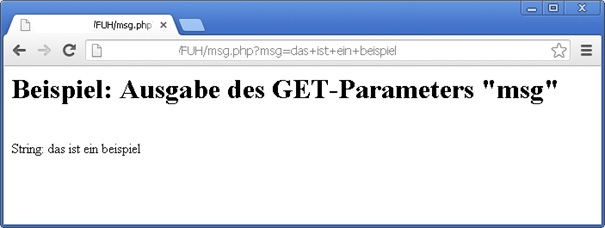
\includegraphics[scale=.75]{abbildungen/xss_1}
 \caption{Ausgabe des eines Beispiel-Strings}
 \label{fig:xss_1} 
\end{figure}

Da im Beispiel keine serverseitige Validierung des Parameters „msg“ vorgenommen wird, ist der Parameter anfällig für Corss-Site-Scripting.
Wird an die URL aus dem vorhergehenden Beispiel JavaScript Code angehängt, wird der Code vom Browser des Anwenders interpretiert und ausgeführt.
\\
\textbf{URL:} http://domain.de/FUH/msg.php?msg=das+ist+ein+beispiel\\<script>alert('XSS')</script>

\begin{figure}[htbp]
 \centering
 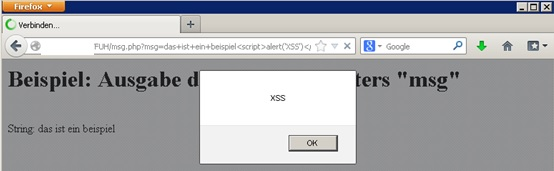
\includegraphics[scale=.75]{abbildungen/xss_2}
 \caption{Der JavaScript-Code kommt im Browser zu Ausführung}
 \label{fig:xss_1} 
\end{figure}

Betrachtet man den Quellcode der Webseite, erkennt man den eingebetteten JavaScript-Code:

\begin{lstlisting}[basicstyle=\ttfamily\footnotesize]
<html>
<body>
<h1>Beispiel: Ausgabe des GET-Parameters "msg"</h1>
<br>
String: das ist ein beispiel<script>alert('XSS')</script></body>
</html>
\end{lstlisting}

\subsubsection{Cross Site Request Forgery}
Bei Cross-Site Request Forgery handelt es sich um eine Angriffstechnik, mit der Daten in der Anwendung unberechtigt verändert werden können. Dabei bringt ein Angreifer den Webbrowser eines bereits authentisierten Benutzers dazu, eine HTTP-Anfrage an die Webanwendung zu stellen. Der Angreifer wählt diese Anfrage so, dass die Webanwendung die ihm gewünschte Funktion (z.B. eine Passwortänderung) ausführt. Sofern das Opfer angemeldet ist und somit bereits über eine gültige Session verfügt, während die HTTP-Anfrage ausgeführt wird, nimmt die Webanwendung die Anfrage entgegen und führt sie mit den Rechten des Opfers aus.

Die Webanwendung kann dabei nicht zwischen HTTP-Anfragen unterscheiden, die korrekt durch den Benutzer initiiert wurde und solchen, die durch CSRF in den Browser des Opfers eingeschleust wurden. Da der Angriff ausschließlich im Webbrowser des Opfers stattfindet und der Angreifer selbst weder aktiv noch passiv mit der Webanwendung interagiert, ist dieser Angriff unmittelbar nur zum Manipulieren von Daten geeignet. Daten direkt auszulesen bzw. mitzulesen ist nicht möglich. Um eine CSRF-Schwachstelle ausnutzen zu können, müssen einige Vorbedingungen erfüllt sein:


\begin{itemize}
      \item Die Webanwendung muss anfällig für CSRF sein
	  \item Das Opfer muss an der Applikation angemeldet sein
	  \item Das Opfer muss dazu gebracht werden, eine HTTP-Anfrage abzusetzen (beispielsweise durch Anklicken eines manipulierten Links
\end{itemize}

Eine Webanwendung ist  anfällig für CSRF, wenn Anfragen an den Webserver statisch sind und keine zufällige Komponente (Token) beinhalten. In diesem Fall können die Anfragen vorab konstruiert und direkt an den Webserver geschickt werden, ohne dass man zuvor die eigentlichen Formulare der Applikation ausgefüllt haben muss.
Im Folgenden ist exemplarisch eine CSRF-Schwachstelle innerhalb der Applikation beschrieben.

